% Autor: Tobias Schwindl

\section{Nachrichten}

\subsection{Nachrichtenseite}

Nicht mit Administratorstatus eingeloggte User können nur die Nachrichten lesen, siehe Graphik \ref{fig:Nachrichten}.

\begin{figure}[!htbp]
 \centering
 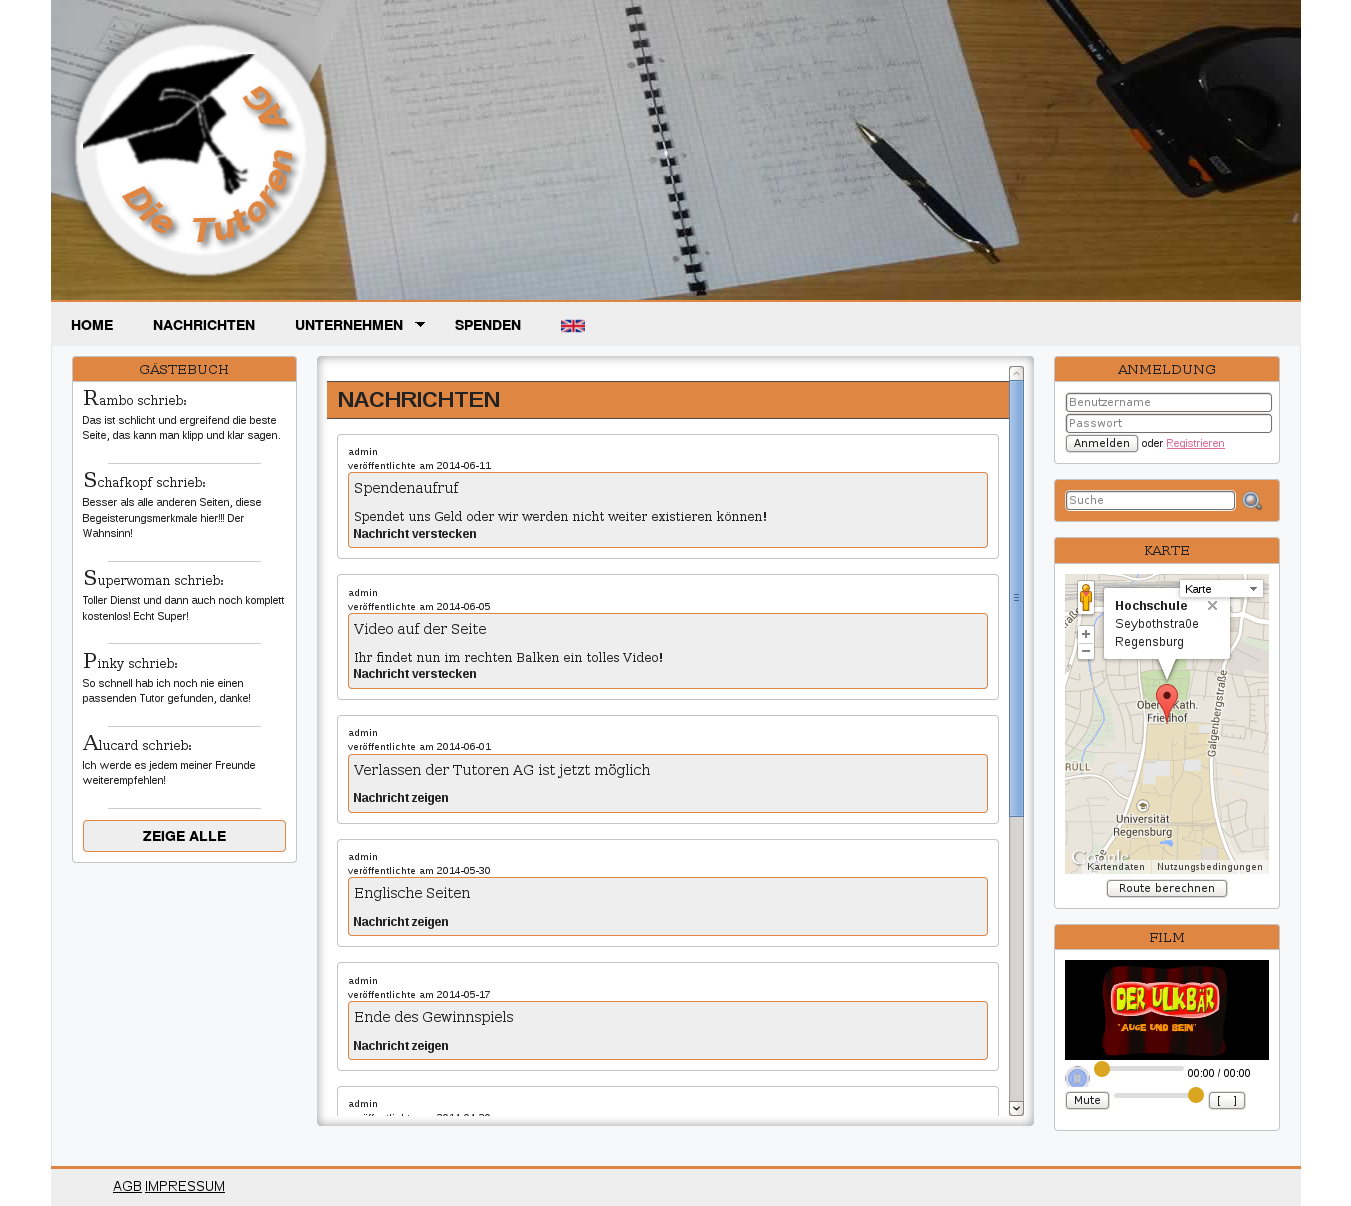
\includegraphics[width=1\textwidth]{../Screenshots/de/Nachrichten}
 \label{fig:Nachrichten}
 \caption{Nachrichtenseite (nicht eingeloggt!)}
\end{figure}

\newpage

\subsection{Als Admin}

Sobald man sich als Administrator angemeldet hat, kann man über das Formular neue Nachrichten hinzufügen, siehe Graphik \ref{fig:Nachrichten_admin}.

\begin{figure}[!htbp]
 \centering
 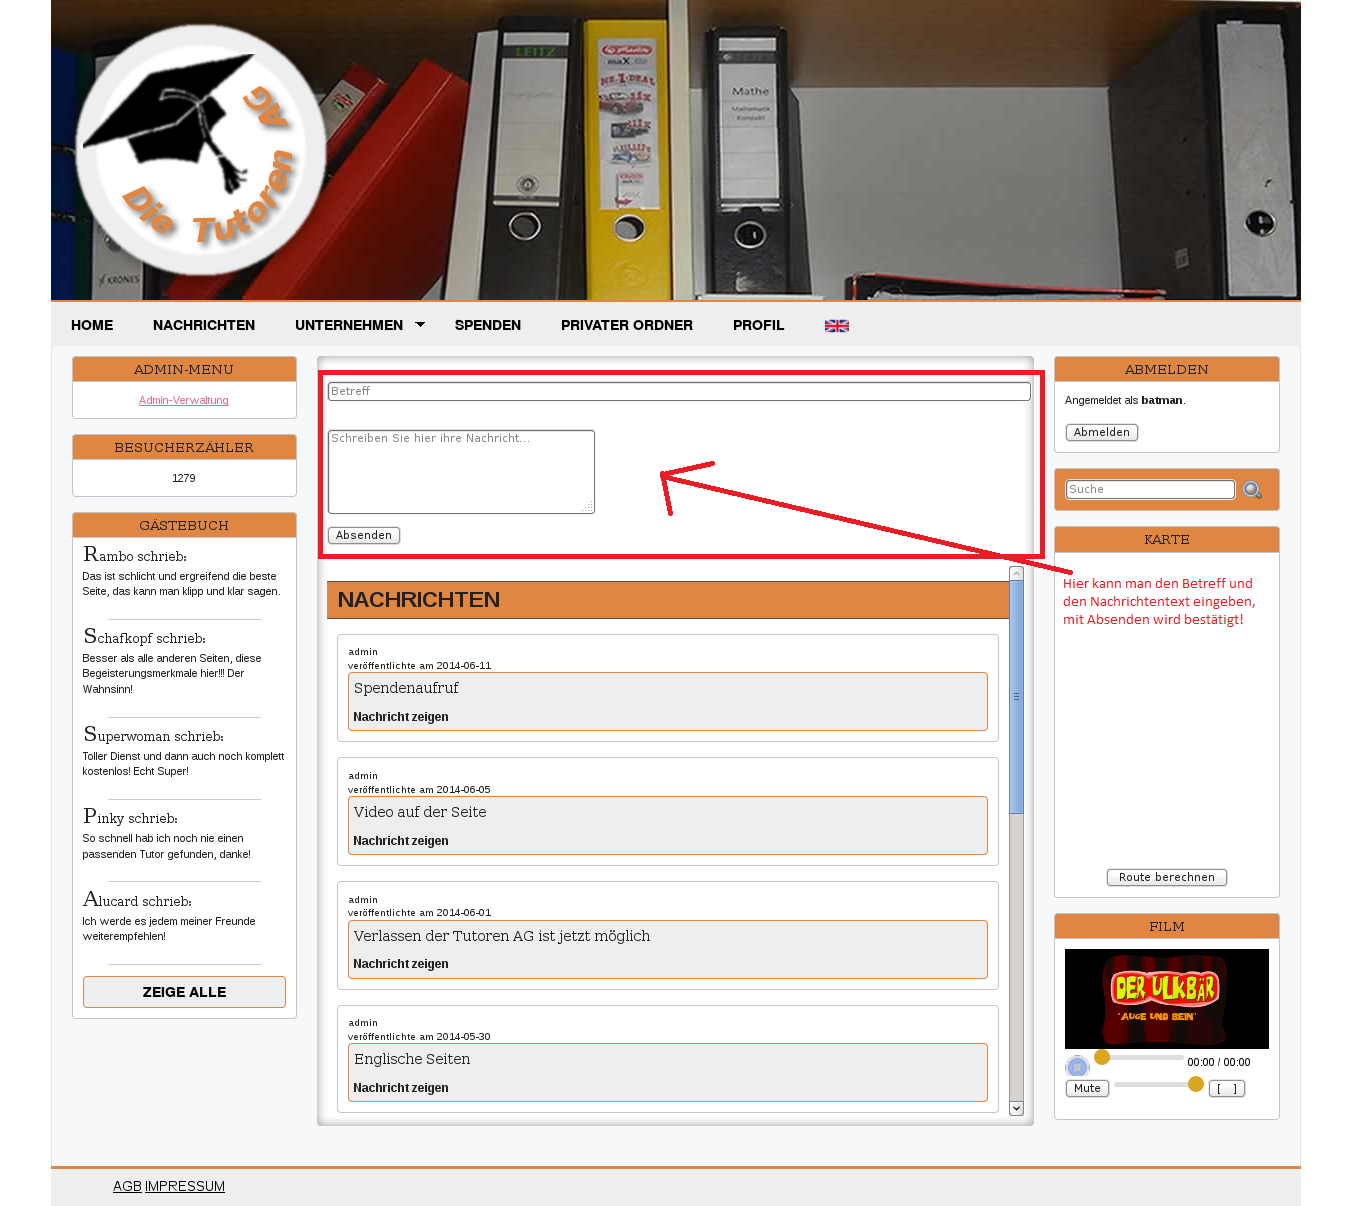
\includegraphics[width=1\textwidth]{../Screenshots/de/Nachrichten_admin}
 \label{fig:Nachrichten_admin}
 \caption{Nachrichtenseite als Admin}
\end{figure}
